\section{Cavern Gamma Simulations}

\par
Although the LZ detector has been constructed underground to limit cosmic radiation, it does come with a drawback of being in a mine with a non-negligibly radioactive rock and the shotcreat and gravel within the David Cavern.
The rate of this has been measured and can be attributed to the shotcreat and gravel. 

One of the most significant sources of background come not from any internal component but rather from $^{238}U$, $^{232}Th$ and $^{40}K$ decays from the cavern in which the LZ detector exists \cite{LZ_Gamma_Ray_Background_ref}.


\begin{figure}[!htbp]
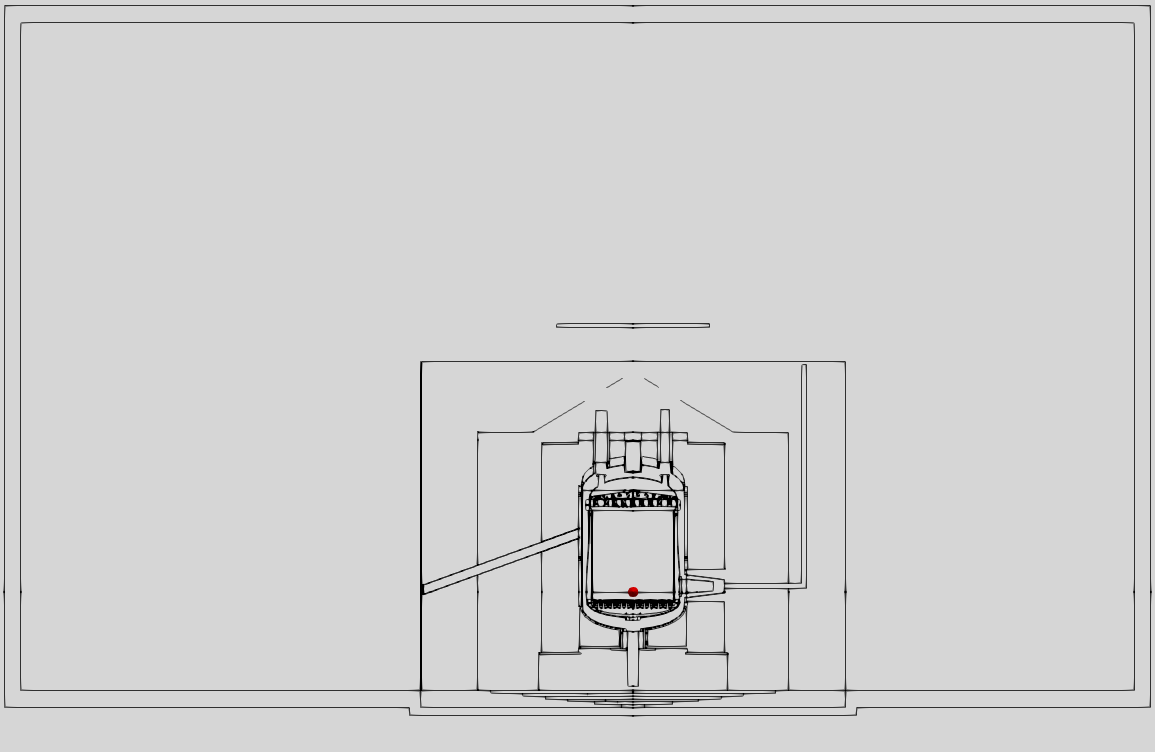
\includegraphics[width=\textwidth]{Figures/Simulations/cavern_geometry_2.png}
\centering
\caption{Cavern Geometry}
\label{fig:Cavern_Geometry}
\end{figure}